\documentclass[tikz,border=6pt]{standalone}
\usepackage{fontspec}
\usepackage{xeCJK}
\setmainfont{Times New Roman}
\setCJKmainfont{Hiragino Sans GB}
\setCJKsansfont{Microsoft YaHei}
\setCJKmonofont{STSong}
\usepackage{xcolor}
\usetikzlibrary{arrows.meta}

\definecolor{axisgray}{HTML}{333333}
\definecolor{lineblue}{HTML}{4A90D9}
\definecolor{linered}{HTML}{E74C3C}

\begin{document}
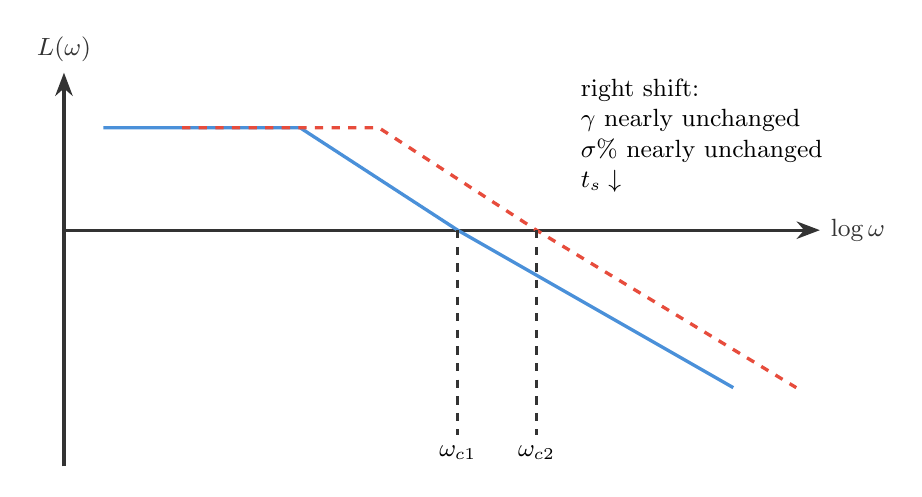
\begin{tikzpicture}[>=Stealth, line width=1.2pt, font=\small]
  \draw[axisgray, ->] (0,0) -- (9.6,0) node[right] {$\log \omega$};
  \draw[axisgray, ->] (0,-3.0) -- (0,2.0) node[above] {$L(\omega)$};
  \draw[lineblue] (0.5,1.3) -- (3.0,1.3) -- (5.0,0.0) -- (8.5,-2.0);
  \draw[linered, dashed] (1.5,1.3) -- (4.0,1.3) -- (6.0,0.0) -- (9.3,-2.0);
  \draw[axisgray, dashed] (5.0,0) -- (5.0,-2.6);
  \draw[axisgray, dashed] (6.0,0) -- (6.0,-2.6);
  \node[below] at (5.0,-2.6) {$\omega_{c1}$};
  \node[below] at (6.0,-2.6) {$\omega_{c2}$};
  \node[align=left] at (8.1,1.2) {right shift:\\$\gamma$ nearly unchanged\\$\sigma\%$ nearly unchanged\\$t_s \downarrow$};
\end{tikzpicture}
\end{document}
